% !TeX root = ../seminar.tex
\section{Gravitational Microlensing}

{\setbeamercolor{background canvas}{bg=black}
\begin{frame}[plain]
\begin{tikzpicture}[remember picture, overlay]
  \node[anchor=east, inner sep=0] at (current page.east)
       {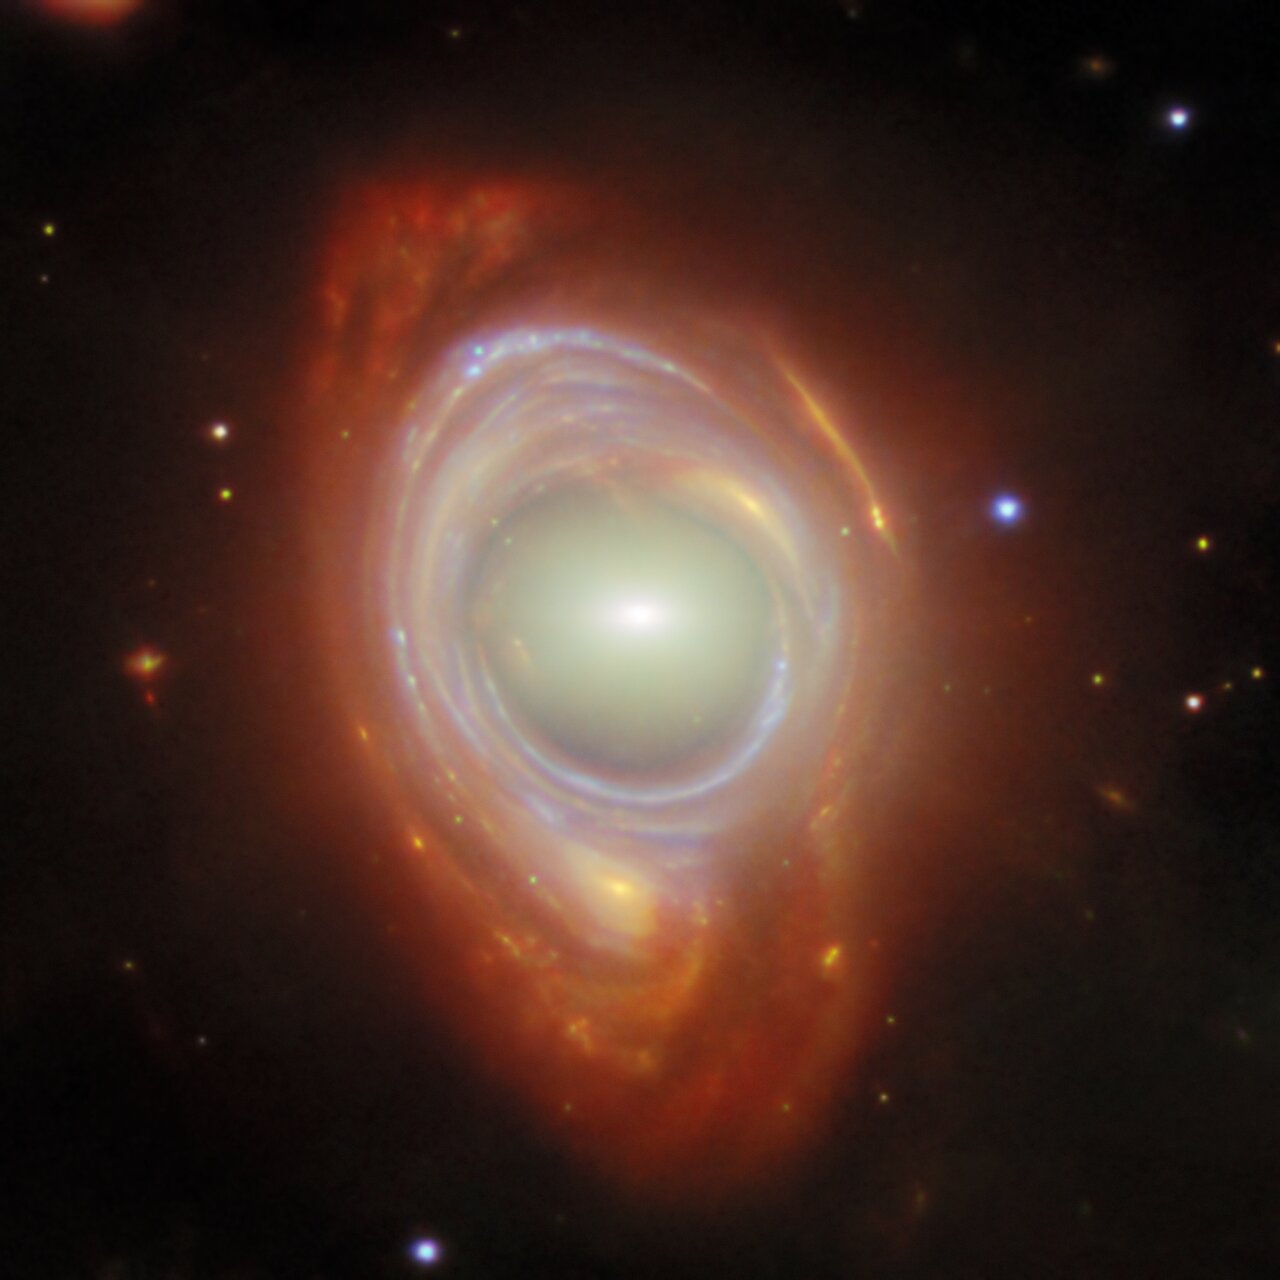
\includegraphics[height=\paperheight]{webb_einstein_ring}};
  \node[anchor=west, text=white, font=\huge\bfseries] at ([xshift=8mm, yshift=8mm]current page.west)
       {Gravity bends light};
  \node[anchor=north west, text=white, align=left, text width=6.2cm] at ([xshift=8mm, yshift=1mm]current page.west)
       {A galaxy \emph{behind} a galaxy,\\ stretched into a ring};
  \node[anchor=north west, text=white, align=left, text width=6.2cm] at ([xshift=8mm, yshift=-12mm]current page.west)
       {\small Our lenses are stars and black holes:\\ the ring is $\sim$\,mas, \textbf{too small to see}};
  \bleedcredit{\href{https://esawebb.org/images/potm2503a/}{ESA/Webb, NASA \& CSA, G.~Mahler (CC BY 4.0)}}
  \bleedsection
\end{tikzpicture}
\note{\begin{itemize}
  \item An Einstein ring imaged by \emph{JWST}: an elliptical galaxy in the cluster SMACSJ0028.2$-$7537 bends the light of a
        spiral far behind it into a near-complete ring.
  \item Galaxy lenses give rings of arcseconds; a star or a black hole gives $\tetE\sim0.5$--$5$\,mas. We do not see the
        ring: we see the star brighten and shift.
\end{itemize}}
\end{frame}}

\begin{frame}{A point lens: two images and the Einstein radius}
\centering
\vspace{1mm}
% Schematic, but the image angles obey the lens equation for beta = 0.06, theta_E = 0.25 (D_S = 10).
\begin{tikzpicture}[x=0.9cm, y=0.62cm, font=\footnotesize]
  \draw[jdlightgrey, dashed] (-0.3,0) -- (10.6,0);
  \draw[jdverylightgrey] (4.2,-2.5) -- (4.2,3.0) node[above, text=jdgrey] {lens plane};
  \draw[jdverylightgrey] (10,-2.5) -- (10,3.0) node[above, text=jdgrey] {source plane};
  % observer, lens, source
  \fill (0,0) circle (2pt) node[below=2pt] {observer};
  \fill[black] (4.2,0) circle (3.5pt);
  \node[below=6pt, fill=white, inner sep=1pt] at (4.2,0) {lens $M$};
  \node[star, star points=5, star point ratio=2.2, fill=yellow!80!orange, draw=orange!70!black,
        inner sep=1.6pt] (S) at (10,0.6) {};
  \node[right=2pt] at (S) {source};
  % the two light paths
  \draw[orange!80!black, thick, -{Latex[length=2mm]}] (10,0.6) -- (4.2,1.184) -- (0,0);
  \draw[orange!80!black, thick, -{Latex[length=2mm]}] (10,0.6) -- (4.2,-0.932) -- (0,0);
  % where the observer sees the images
  \uncover<2->{
  \draw[orange!80!black, dotted, thick] (0,0) -- (10,0.6);
  \draw[jdblue, densely dashed] (4.2,1.184) -- (10,2.818);
  \draw[jdblue, densely dashed] (4.2,-0.932) -- (10,-2.218);
  \node[star, star points=5, star point ratio=2.2, fill=yellow!40, draw=orange!50, inner sep=1.3pt]
       at (10,2.818) {};
  \node[star, star points=5, star point ratio=2.2, fill=yellow!40, draw=orange!50, inner sep=0.9pt]
       at (10,-2.218) {};
  \node[right=3pt, text=jdblue] at (10,2.818) {image $+$};
  \node[right=3pt, text=jdblue] at (10,-2.218) {image $-$};
  % angles at the observer
  \draw[jdblue] (1.6,0) arc (0:15.8:1.6);
  \node[text=jdblue] at (1.95,0.27) {$\theta$};
  \draw[orange!80!black] (2.8,0) arc (0:3.4:2.8);
  \node[text=orange!80!black] at (3.12,0.1) {$\beta$};}
  % distances
  \draw[{Latex[length=1.6mm]}-{Latex[length=1.6mm]}] (0,-2.0) -- node[fill=white, inner sep=1pt] {$D_L$} (4.2,-2.0);
  \draw[{Latex[length=1.6mm]}-{Latex[length=1.6mm]}] (0,-2.55) -- node[fill=white, inner sep=1pt] {$D_S$} (10,-2.55);
\end{tikzpicture}

\vspace{3mm}
\uncover<3->{%
\[
  \beta = \theta - \frac{\tetE^2}{\theta}
  \qquad\qquad
  \tetE = \sqrt{\kappa\,M\,\pirel}
\]
{\small\color{jdgrey} $\kappa = 8.14$\,mas$/\Msun$, \quad $\pirel = {\rm AU}\,(1/D_L - 1/D_S)$: the lens--source parallax}\par}
\vspace{1mm}
\uncover<4->{bulge star: $\tetE\approx0.4$\,mas \qquad black hole: $\tetE\approx5$\,mas, images $\gtrsim10$\,mas apart}
\vfill
\refnote{\ads{1986ApJ...304....1P}{Paczy\'nski 1986, ApJ 304, 1}}
\note{\begin{itemize}
  \item Images at $\theta_\pm = \tfrac{\tetE}{2}\bigl(u\pm\sqrt{u^2+4}\bigr)$, $u=\beta/\tetE$.
  \item $\kappa = 8.144\,{\rm mas}/\Msun$, $\pirel = {\rm AU}(1/D_L-1/D_S)$.
  \item Bulge star: $0.5\,\Msun$, $D_L=6$, $D_S=8$\,kpc. Black hole: $10\,\Msun$ at $2$\,kpc.
  \item The two images are $\sim2\tetE$ apart: usually far too close to separate.
\end{itemize}}
\end{frame}

\begin{frame}{A lens crossing a star}
\centering
\vspace{2mm}
\animategraphics[autoplay, loop, controls=off, poster=40, width=.76\linewidth]{16}{img/anim/frame_}{00}{80}

\vspace{4mm}
We see only the \textbf{total light} (top: \textbf{photometry})\\ and where its \textbf{centre} lies (bottom: \textbf{astrometry})
\vfill
\refnote{Reverse ray tracing of a limb-darkened star, $R_\star=0.6\,\tetE$ (A.~Salehi); the curves are
measured from the traced images.}
\note{\begin{itemize}
  \item In a real event the images are too close to separate: a telescope sees only their total light and its centre.
  \item Near the peak the lens is \emph{inside} the stellar disc: an Einstein ring forms, the finite source caps the
        magnification and reverses the centroid shift. Dashed grey: a point source.
\end{itemize}}
\end{frame}

\begin{frame}{Two observables: photometry and astrometry}
\vspace{1mm}
\centering
The two images are $\sim2\tetE$ apart: usually unresolved, seen as one blended star
\vspace{1mm}
\begin{columns}[T]
\begin{column}{.47\linewidth}
\centering
\textbf{Photometry}: \emph{how bright?}\\
{\small the star's flux vs.\ time (the light curve)}
\[
  A(u) = \frac{u^2+2}{u\sqrt{u^2+4}}
\]
\uncover<2->{%
\[
  \tE = \frac{\tetE}{\mu_{\rm rel}}
\]
mixes \textbf{mass}, \textbf{distance}, \textbf{velocity}}
\end{column}
\begin{column}{.47\linewidth}
\centering
\uncover<3->{%
\textbf{Astrometry}: \emph{where?}\\
{\small the light centre's position on the sky vs.\ time}
\[
  \delta\theta = \frac{\tetE\,u}{u^2+2}
\]
\[
  \delta\theta_{\max} = \frac{\tetE}{\sqrt8}\quad\text{at } u=\sqrt2
\]
measures $\tetE$ directly}
\end{column}
\end{columns}
\vfill
{\centering\small\color{jdgrey} $u$: lens--source separation in units of $\tetE$; \quad $\mu_{\rm rel}$: their relative proper motion\par}
\vspace{1mm}
\refnote{\ads{1986ApJ...304....1P}{Paczy\'nski 1986, ApJ 304, 1};
\ads{2000ApJ...542..785G}{Gould 2000, ApJ 542, 785}}
\note{\begin{itemize}
  \item $u(t) = \sqrt{u_0^2 + ((t-t_0)/\tE)^2}$: impact parameter $u_0$, peak time $t_0$.
  \item The timescale is the one physical quantity a simple light curve gives. Bulge events: $\tE\sim20$\,d;
        black holes: hundreds of days.
  \item The centroid shift peaks $\sim1.4\,\tE$ from the photometric peak, often in a different Roman season.
  \item The images are $\Delta\theta=\tetE\sqrt{u^2+4}\ge2\tetE$ apart: $\gtrsim10$\,mas for tens of $\Msun$ at a few kpc,
        so for heavy, nearby lenses they may be resolved.
\end{itemize}}
\end{frame}

\begin{frame}{Microlensing parallax: a second viewpoint}
\vspace{1mm}
\centering
\begin{tikzpicture}[font=\footnotesize, x=1cm, y=1cm]
  % left: annual parallax (Earth's orbit makes the track wiggle)
  \begin{scope}
    \draw[jdlightgrey, fill=jdverylightgrey!40] (0,0) circle (1.1);
    \fill (0,0) circle (2pt) node[below left=-1pt] {lens};
    \node[text=jdgrey, font=\scriptsize] at (0,1.35) {Einstein ring};
    \draw[orange!80!black, dashed, -{Latex}] (-2.3,0.35) -- (2.3,0.35);
    \uncover<2->{\draw[orange!80!black, very thick, -{Latex}, domain=-2.3:2.3, samples=80]
         plot (\x, {0.35+0.28*sin(deg(2.6*\x))});
    \node[align=center, font=\small] at (0,-1.85) {\textbf{annual}: Earth's orbit\\ \footnotesize needs a long event};}
  \end{scope}
  % right: satellite parallax (Earth and L2 see different tracks)
  \uncover<3->{
  \begin{scope}[xshift=6.0cm]
    \draw[jdlightgrey, fill=jdverylightgrey!40] (0,0) circle (1.1);
    \fill (0,0) circle (2pt);
    \draw[jdblue, very thick, -{Latex}] (-2.3,0.25) -- (2.3,0.25) node[right] {Earth};
    \draw[red!70!black, very thick, -{Latex}] (-2.3,0.65) -- (2.3,0.65) node[right] {L2};
    \draw[{Latex[length=1.3mm]}-{Latex[length=1.3mm]}] (-1.75,0.25) -- node[left=1pt] {$\Delta u$} (-1.75,0.65);
    \node[align=center, font=\small] at (0,-1.85) {\textbf{satellite}: Roman vs.\ Rubin\\ \footnotesize works for short events too};
  \end{scope}}
\end{tikzpicture}

\vspace{1mm}
\[
  \piE = \frac{\pirel}{\tetE}
  \qquad
  \uncover<2->{\vec u(t) = \vec u_0 + \frac{t-t_0}{\tE}\,\hat{\vec\mu} + \piE\,\vec s(t)}
  \qquad
  \uncover<3->{\Delta u \simeq \piE\,\frac{D_\perp}{\rm AU}}
\]
\uncover<4->{Black hole: $\piE=\sqrt{\pirel/\kappa\Ml}$ is \textbf{small} $\Rightarrow$ a small, slow wiggle}
\vfill
\refnote{\ads{1966MNRAS.134..315R}{Refsdal 1966, MNRAS 134, 315};
\ads{1992ApJ...392..442G}{Gould 1992, ApJ 392, 442};
\ads{2000ApJ...542..785G}{Gould 2000, ApJ 542, 785}}
\note{\begin{itemize}
  \item Parallax: the same lens--source pair seen from a different place lines up differently. $\piE$ is the relative
        parallax $\pirel={\rm AU}(1/D_L-1/D_S)$ in units of $\tetE$: one AU of observer motion moves the track by
        $\piE$ Einstein radii.
  \item Annual: $\vec s(t)$ = Earth's (or Roman's) displacement from uniform motion, in AU, projected on the sky.
        It needs $\tE$ to be a sizeable fraction of a year: black holes qualify.
  \item Satellite: two observers $D_\perp$ apart see the peak at different times and heights, at the same moment,
        so it needs no long event (as with \emph{Spitzer}). Roman (L2) and Earth: $D_\perp\approx0.01$\,AU, so
        $\Delta u\approx0.01\,\piE$.
  \item The expectation going in: Roman + Rubin give a satellite parallax. The results test it.
  \item Black hole, $10\,\Msun$ at $2$\,kpc, source at $8$\,kpc: $\piE\approx0.05$.
\end{itemize}}
\end{frame}

\begin{frame}{From observables to a lens mass}
\centering
\vspace{2mm}
\begin{tikzpicture}[font=\small,
    ob/.style={terminator, fill=orange!15, text width=2.6cm, align=center, minimum height=3.2em},
    qu/.style={terminator, fill=blue!10, text width=4.4cm, align=center, minimum height=3em},
    re/.style={terminator, fill=green!15, text width=3.0cm, align=center, minimum height=3em}]
  \node[ob] (ph) at (0,1.1) {\textbf{Photometry}};
  \node[ob] (as) at (0,-1.1) {\textbf{Astrometry}};
  \node[qu] (te) at (4.9,1.9) {$\tE$, $u_0$, $t_0$: the shape};
  \uncover<2->{\node[qu] (pi) at (4.9,0) {$\piE$: the parallax};}
  \uncover<3->{\node[qu] (th) at (4.9,-1.9) {$\tetE$: the centroid's excursion};}
  \uncover<4->{
  \node[re] (m) at (9.9,0.85) {\textbf{Lens mass}\\ $\Ml = \dfrac{\tetE}{\kappa\,\piE}$};
  \node[re] (d) at (9.9,-1.05) {\textbf{Distance}\\ $\pirel = \tetE\,\piE$};}
  \path[connector] (ph.east) -- (te.west);
  \uncover<2->{\path[connector] (ph.east) -- (pi.west); \path[connector] (as.east) -- (pi.west);}
  \uncover<3->{\path[connector] (as.east) -- (th.west);}
  \uncover<4->{
  \path[connector] (pi.east) -- (m.west); \path[connector] (th.east) -- (m.west);
  \path[connector] (pi.east) -- (d.west); \path[connector] (th.east) -- (d.west);}
\end{tikzpicture}

\vspace{5mm}
\uncover<5->{%
\[
  \left(\frac{\sigma_M}{M}\right)^2 = \left(\frac{\sigma_{\piE}}{\piE}\right)^2 + \left(\frac{\sigma_{\tetE}}{\tetE}\right)^2
\]
Black holes: $\tetE$ large (easy), $\piE$ small (hard)}
\vfill
\refnote{\ads{2000ApJ...542..785G}{Gould 2000, ApJ 542, 785}}
\note{\begin{itemize}
  \item $\piE = \pirel/\tetE$: from the light curve's distortion by Earth's orbit (annual parallax), or from two
        observers at once (satellite parallax: Roman at L2, Rubin on Earth, $0.01$\,AU apart).
  \item $\tetE$: from the size of the centroid's excursion, or from the separation of the two images.
\end{itemize}}
\end{frame}

{\setbeamercolor{background canvas}{bg=black}
\begin{frame}[plain]
\begin{tikzpicture}[remember picture, overlay]
  \node[anchor=north, inner sep=0] (im) at (current page.north)
       {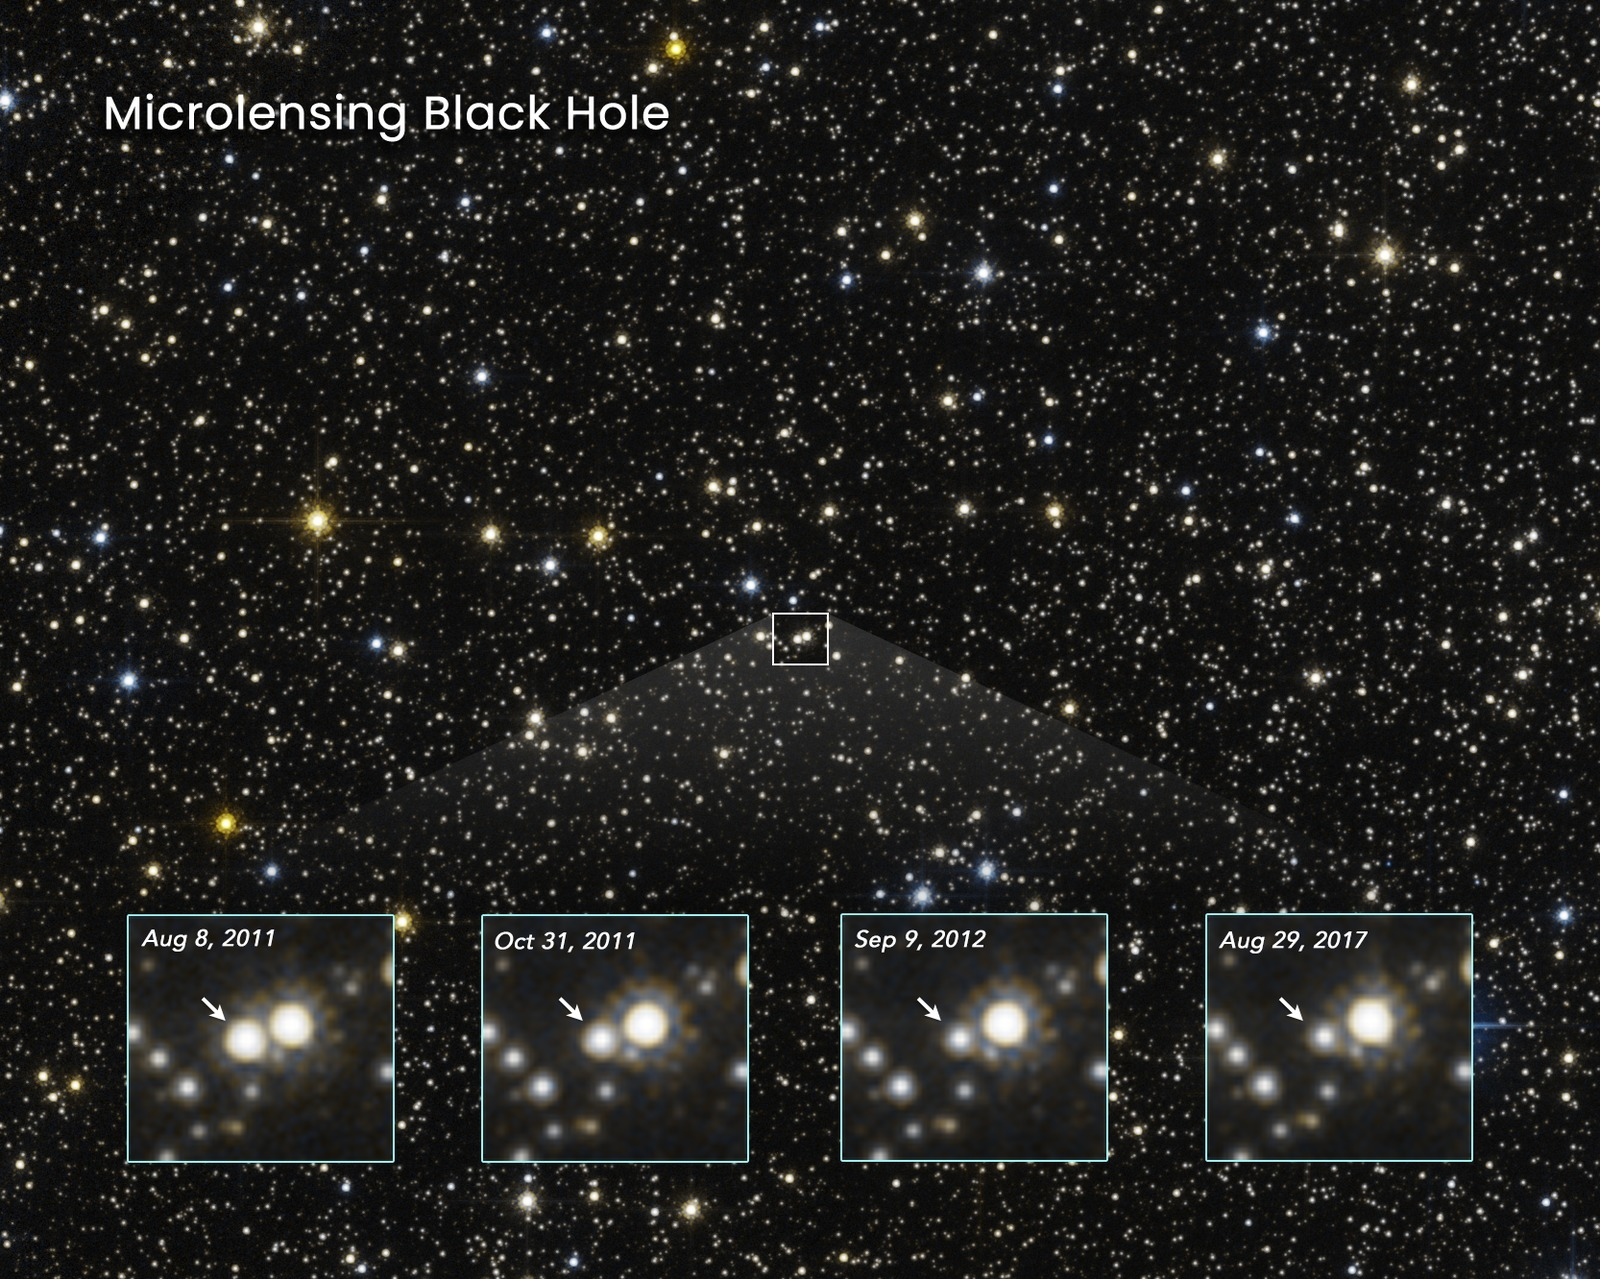
\includegraphics[height=.88\paperheight]{stsci_isolated_bh}};
  \node[anchor=north, text=white, font=\normalsize] at ([yshift=-1mm]im.south)
       {2011--2017: \emph{Hubble} watches a star brighten and fade, lensed by \textbf{something unseen}};
  \bleedcredit{\href{https://www.astropix.org/image/stsci/2022-01b}{NASA, ESA, K.~Sahu (STScI)}}
\end{tikzpicture}
\note{\begin{itemize}
  \item Real \emph{HST} (WFC3/UVIS) data: a field toward the Galactic centre, and the source star of OGLE-2011-BLG-0462
        (arrow) in four epochs, bright in August 2011 and back to normal by 2017.
  \item The astrometric shift, $\sim1$\,mas, is a fraction of a pixel: not visible here, but measured from the
        star's position at each epoch.
  \item No light from the lens: an isolated, dark, compact object.
\end{itemize}}
\end{frame}}

\begin{frame}{The first isolated black hole: OGLE-2011-BLG-0462}
\vspace{1mm}
\begin{columns}[T]
\begin{column}{.38\linewidth}
\centering
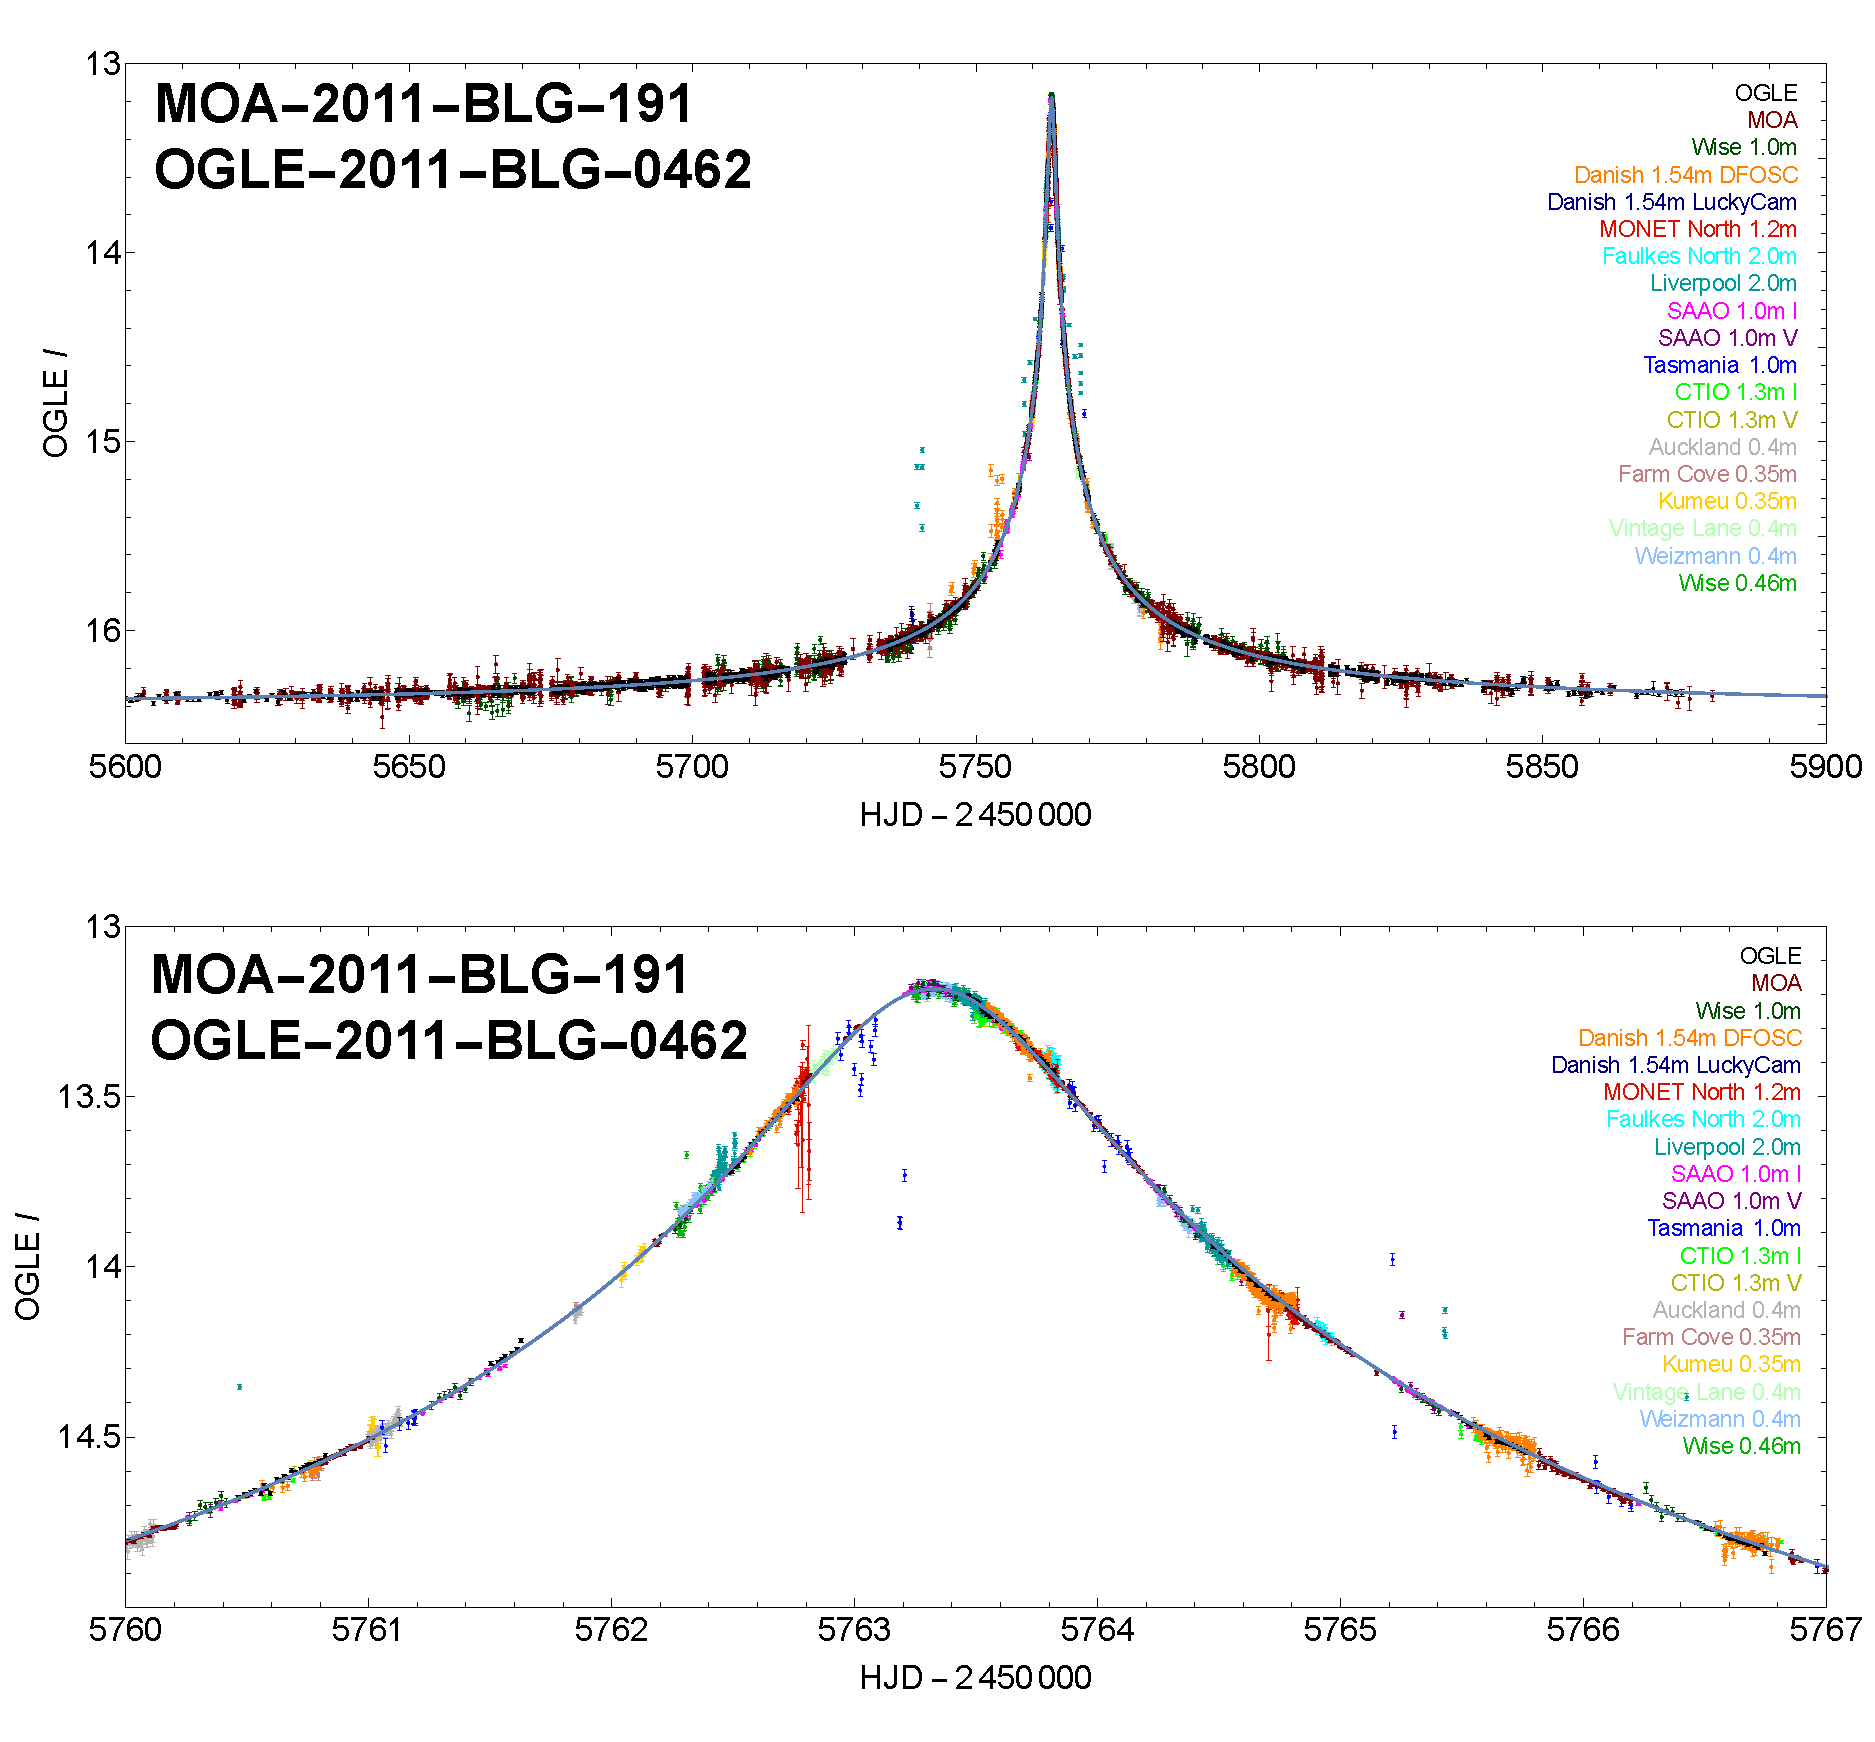
\includegraphics[width=.92\linewidth]{sahu2022_photometry}
\end{column}
\begin{column}{.24\linewidth}
\centering
\vspace{2mm}
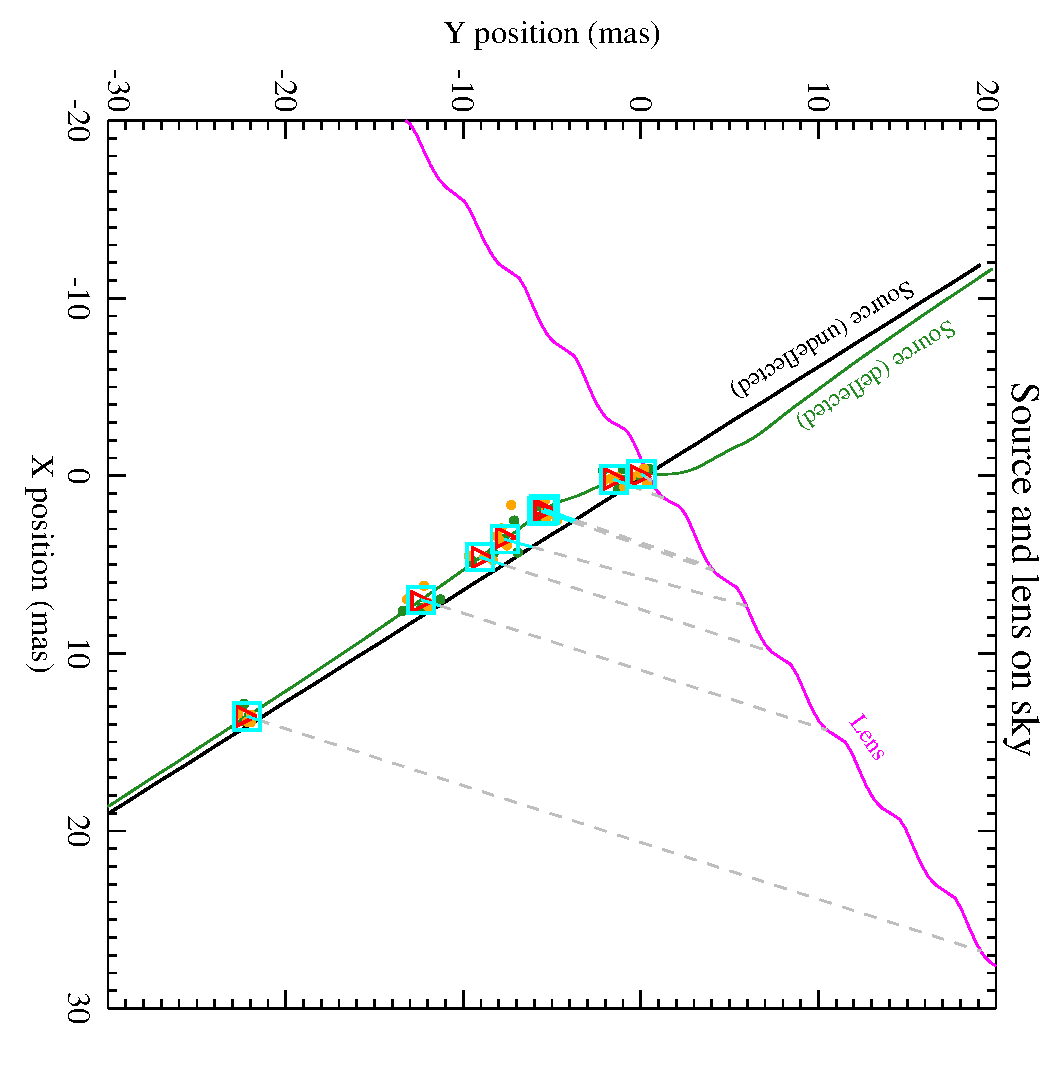
\includegraphics[angle=90,width=.9\linewidth]{sahu2022_sky}
\end{column}
\begin{column}{.34\linewidth}
\begin{itemize}\setlength{\itemsep}{6pt}
  \item<+-> Photometry: $\tE\approx270$\,d,\\ $\piE$ from the ground
  \item<+-> Astrometry: \emph{HST}, 6 years\\ $\to\tetE\approx5$\,mas
  \item<+-> $\Ml = 7.1\pm1.3\,\Msun$\\ at $1.6$\,kpc
\end{itemize}
\end{column}
\end{columns}
\vspace{2mm}
\credit{\ads{2022ApJ...933...83S}{Sahu et al.\ 2022, ApJ 933, 83}}
\vfill
\uncover<4->{%
\begin{beamercolorbox}[rounded=true,sep=6pt,wd=\linewidth]{block body alerted}
\centering
The first \textbf{dark} object weighed by its gravity alone:\\
both observables together \textbf{work}
\end{beamercolorbox}}
\vfill
\note{\begin{itemize}
  \item Sahu et al.\ 2022: a decade-long \emph{HST} programme following up long ground-based events.
  \item Left: the light curve (OGLE, MOA, \ldots) and its parallax distortion. Right: the source's measured
        position over 6 years, deflected by $\sim1$\,mas.
  \item $\tetE\approx5.2$\,mas and $\piE\approx0.09$: $\Ml = \tetE/(\kappa\piE)\approx7\,\Msun$, no light from the lens
        $\to$ a black hole. Isolated: no companion in the data.
  \item Its transverse velocity ($\sim45$\,km/s relative to the disc) hints at a natal kick.
\end{itemize}}
\end{frame}

\begin{frame}{\ldots but how heavy is it?}
\vspace{1mm}
\begin{columns}[c]
\begin{column}{.50\linewidth}
\centering
% published masses of the lens, linear axis 0-10 Msun, 0.6 cm per Msun
\begin{tikzpicture}[x=0.5cm, y=0.62cm, font=\footnotesize]
  \fill[orange!25] (1.1,-0.4) rectangle (2.3,4.6);
  \node[anchor=south, align=center, font=\scriptsize] at (1.7,4.6) {neutron\\ stars};
  \fill[jdblue!12] (5,-0.4) rectangle (10,4.6);
  \node[anchor=south, font=\scriptsize] at (7.5,4.6) {black holes};
  \draw[-{Latex}] (0,-0.4) -- (10.3,-0.4);
  \foreach \m in {0,2,...,10} \draw (\m,-0.4) -- (\m,-0.55) node[below] {\m};
  \node[below] at (5,-1.05) {lens mass [$\Msun$]};
  {\draw[jdblue!80!black, very thick, {|-|}] (5.8,3.9) -- (8.4,3.9); \fill[jdblue!80!black] (7.1,3.9) circle (2.5pt);
    \node[anchor=east, font=\tiny] at (-0.2,3.9) {Sahu+ 2022};}
  \uncover<2->{\draw[red!70!black, very thick, {|-|}] (1.6,2.8) -- (4.4,2.8);
    \node[anchor=east, font=\tiny] at (-0.2,2.8) {Lam+ 2022};}
  \uncover<4->{\draw[jdblue!80!black, very thick, {|-|}] (7.06,1.5) -- (8.70,1.5); \fill[jdblue!80!black] (7.88,1.5) circle (2.5pt);
    \node[anchor=east, font=\tiny] at (-0.2,1.5) {Mr\'oz+ 2022};
    \draw[jdblue!80!black, very thick, {|-|}] (4.98,0.4) -- (7.22,0.4); \fill[jdblue!80!black] (6.03,0.4) circle (2.5pt);
    \node[anchor=east, font=\tiny] at (-0.2,0.4) {Lam \& Lu 2023};}
\end{tikzpicture}
\end{column}
\begin{column}{.46\linewidth}
\begin{itemize}\setlength{\itemsep}{6pt}
  \item<2-> Same event, nearly the same data:\\ black hole \emph{or} neutron star?
  \item<3-> \textbf{Systematics}, not noise:\\ in $\piE$ (ground) and $\tetE$ (\emph{HST})
  \item<4-> Settled only by re-analysis:\\ a $\sim7\,\Msun$ black hole
\end{itemize}
\end{column}
\end{columns}
\vfill
\uncover<5->{%
\begin{beamercolorbox}[rounded=true,sep=6pt,wd=\linewidth]{block body alerted}
\centering
$\Ml=\tetE/\kappa\piE$: a bias in \emph{either} observable goes straight into the mass.\\
For a black hole $\piE$ is small and easily biased $\Rightarrow$ measure it robustly
\end{beamercolorbox}}
\vfill
\refnote{%
\ads{2022ApJ...933...83S}{Sahu et al.\ 2022, ApJ 933, 83};
\ads{2022ApJ...933L..23L}{Lam et al.\ 2022, ApJL 933, L23};
\ads{2022ApJ...937L..24M}{Mr\'oz, Udalski \& Gould 2022, ApJL 937, L24};
\ads{2023ApJ...955..116L}{Lam \& Lu 2023, ApJ 955, 116}}
\note{\begin{itemize}
  \item Lam et al.\ 2022 analysed similar photometry and \emph{HST} astrometry and found $1.6$--$4.4\,\Msun$: a neutron
        star could not be excluded.
  \item The difference lay in the systematics: the ground-based parallax (which data sets, how their errors are
        treated) and the reduction of the \emph{HST} images.
  \item Mr\'oz, Udalski \& Gould 2022 re-derived the parallax from OGLE photometry; Lam \& Lu 2023 re-analysed with more
        \emph{HST} epochs. Both: a black hole.
  \item Lessons for this thesis: the mass needs \emph{both} $\piE$ and $\tetE$, and a single event's mass can move by a
        factor $\sim2$. A robust $\piE$ is the crux: how well Roman (and Rubin) can measure it is what the forecast must
        tell us.
\end{itemize}}
\end{frame}

\begin{frame}{Black holes stand out in the microlensing observables}
\vspace{1mm}
\begin{columns}[c]
\begin{column}{.60\linewidth}
\centering
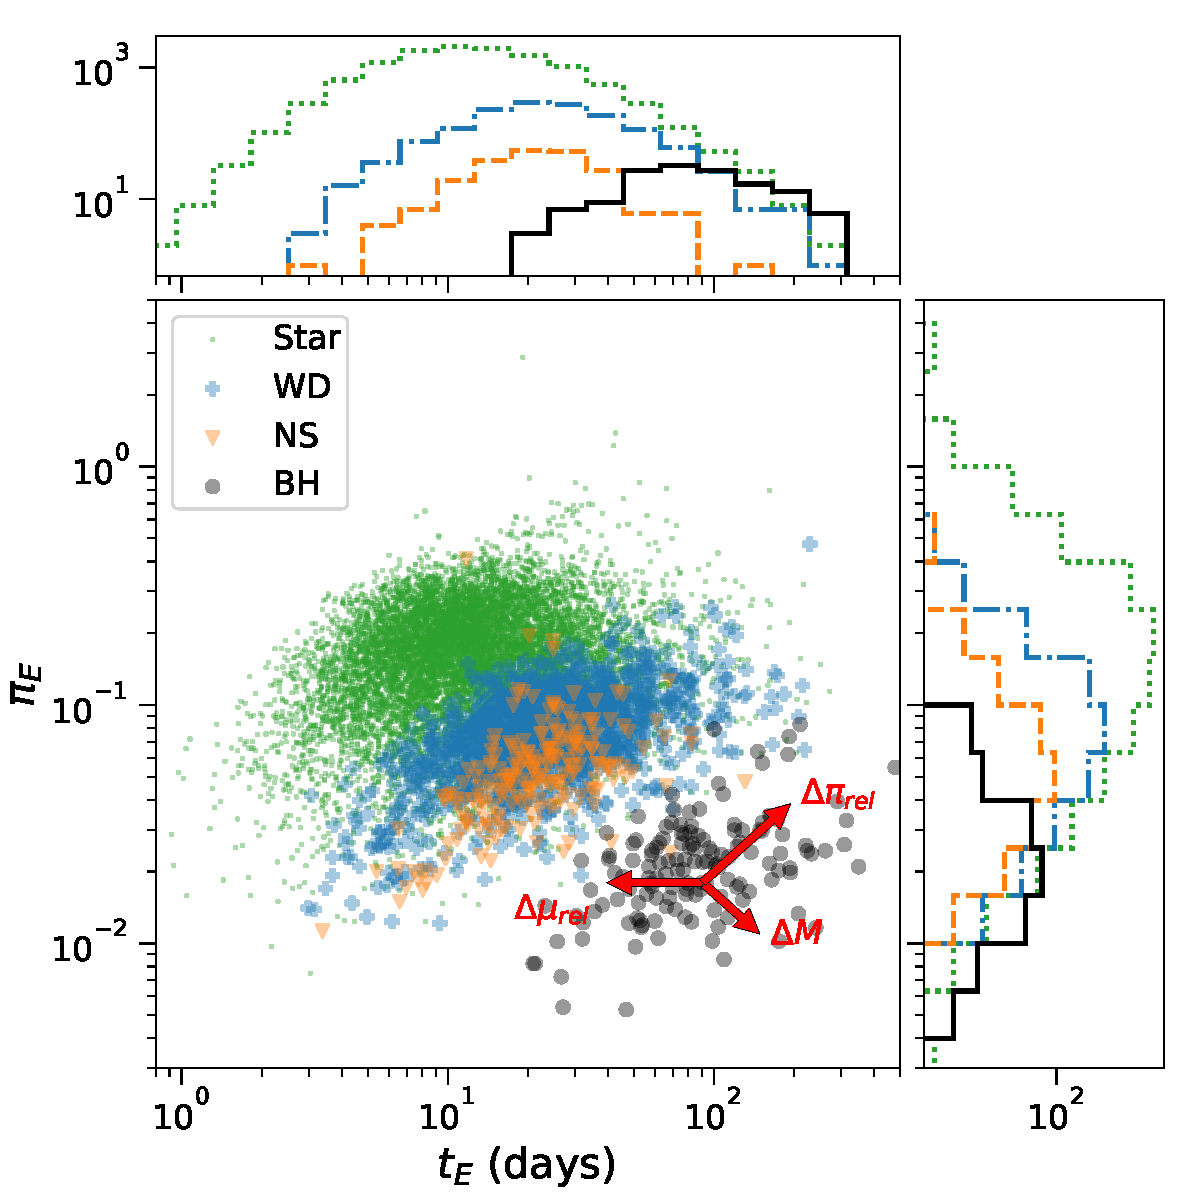
\includegraphics[width=.48\linewidth]{lam2020_tE_piE}\hspace{2mm}%
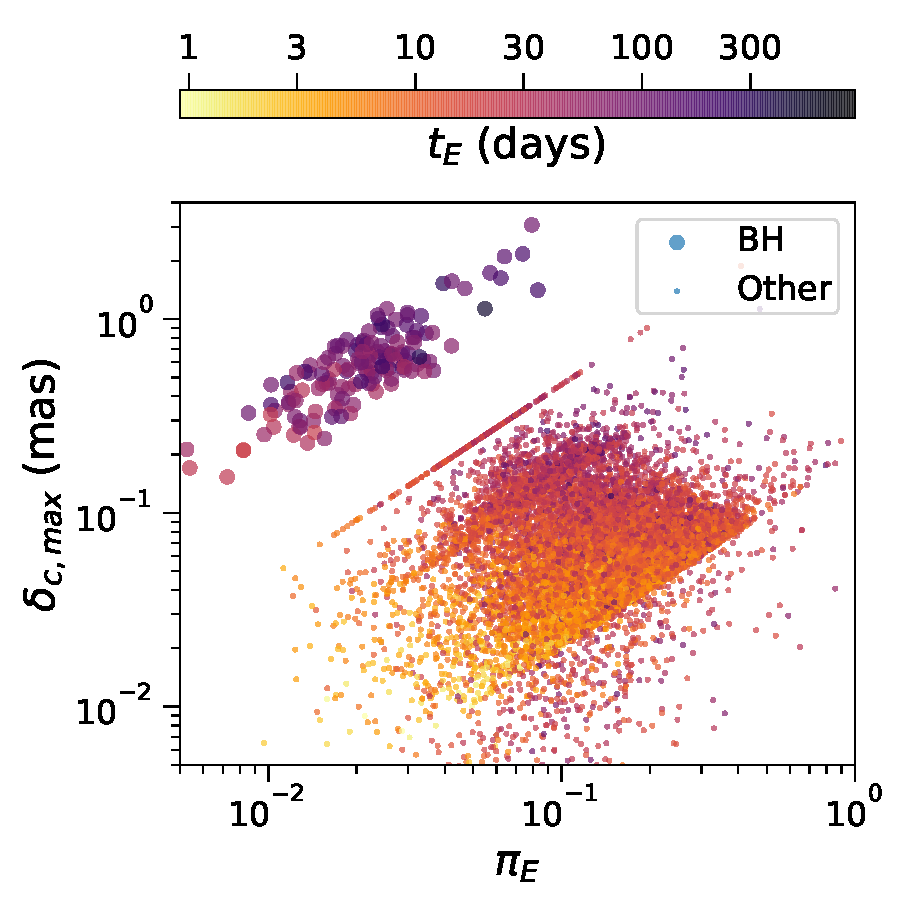
\includegraphics[width=.48\linewidth]{lam2020_deltac_piE}\\[2mm]
\credit{\ads{2020ApJ...889...31L}{Lam et al.\ 2020, ApJ 889, 31} (PopSyCLE)}
\end{column}
\begin{column}{.36\linewidth}
Black holes have
\begin{itemize}\setlength{\itemsep}{4pt}
  \item a \textbf{long} $\tE$
  \item a \textbf{small} $\piE$
  \item a \textbf{large} centroid shift
\end{itemize}
\vspace{6mm}
\uncover<2->{Long, heavy events:\\ \textbf{Roman} and \textbf{Rubin} will see them}
\end{column}
\end{columns}
\vfill
\refnote{\ads{2023ApJ...955..116L}{Lam \& Lu 2023, ApJ 955, 116}}
\note{\begin{itemize}
  \item PopSyCLE simulation of bulge events: black holes (BH) separate from stars, white dwarfs and neutron stars.
  \item Lam \& Lu 2023 predict that Roman, with HST-like astrometry over a far larger field, will measure the masses of
        hundreds of isolated black holes. Roman and Rubin have each been forecast alone; the next section shows what
        is missing: both, on the same events.
\end{itemize}}
\end{frame}
